\section{System Architecture}\label{sec:architecture}

This section describes how the system is built: the offline data pipeline that produces the
embedded catalogue, the components that make up the conversational loop, the lifecycle of a single
turn, and the interfaces through which the system is driven.

\subsection{Data Pipeline}

The movie catalog is constructed from The Movie Database (TMDB) through a reproducible, multi-modal ingestion pipeline.
To transform raw entertainment metadata into a vector-optimized database, the pipeline processes the source data across three main stages, after which the fully embedded catalog is partitioned into three slices for downstream use: a held-out evaluation set, a main operational set, and a compact development set.

\paragraph{Scrape:} Ingestion begins by downloading TMDB's daily catalog export.
To maintain data quality and processing efficiency, the pipeline immediately discards adult content and applies a popularity threshold before initiating detailed API requests.
The surviving titles are enriched with credits, user reviews, keywords, and trailer links. 

\paragraph{Embed:} Each movie is encoded into dense vectors across three distinct modalities.
First, a \textbf{composite text} (title, synopsis, genres, cast, director, and keywords) is encoded with the \emph{BAAI BGE-large-en-v1.5} sentence-embedding model into a 1024-dimensional, $\ell_2$-normalized vector.
Then, the aggregated \textbf{user review text} (only top reviews) is encoded by the same model into the same 1024-dimensional space.
Finally, the \textbf{visual modality} is captured by sampling evenly spaced frames from the movie's trailer, embedding them with the \emph{OpenCLIP ViT-H/14} vision encoder, and mean-pooling them into a single 1024-dimensional vector.

\paragraph{Fuse:} Because the textual and visual encoders inhabit entirely different semantic vector spaces, the pipeline employs two distinct fusion strategies.
Text and review embeddings are merged directly via a weighted average of their vectors since they share a underlying space.
In contrast, the text and trailer modalities are fused at the distance level using a weighted sum of their respective cosine-distance matrices, combining their structural signals without forcing them into an artificial, unified space.

\subsection{Architectural Overview}

The system is a small set of single-purpose components coordinated around one orchestrator (Figure~\ref{fig:architecture}). 
The subsections below describe each component, their purposes, and context.

\begin{figure*}[tp]
  \centering
  
\includegraphics[width=0.68\textwidth]{figures/architecture_diagram.pdf}
  \caption{System components and the path of a single turn. The oracle's message enters the
  deterministic \textbf{Coordinator}, which routes it through read-only agents.}
  \label{fig:architecture}
\end{figure*}

\paragraph{Coordinator:} The \textbf{deterministic} orchestrator of the system, acting as both the session handler and the turn workflow manager.
As the only writer of state and the sole component that communicates directly with the oracle, it directs the system's execution during each turn and provides the necessary context to each downstream agent.
The coordinator maintains \textbf{no in-memory session state}; instead, it reloads the current snapshot and re-reads the database at every turn, ensuring its behavior depends entirely on the persisted dialogue history.

\paragraph{Intent Agent:} The \textbf{strong-model} parser that maps the oracle's free-form message onto an \textbf{ordered list of actions}, each with a confidence score and operation parameters.
Rather than operating on raw embeddings, it evaluates the message against rich contextual signals, reading the user's input alongside the recent dialogue transcript, pending clarifier questions, and the current cluster labels and summaries.
Every action is drawn from a fixed, closed vocabulary, split into \textbf{navigation} operations that reshape the clustering and \textbf{dialogue} moves that do not:
\begin{itemize}[leftmargin=1.4em]
  \item \textbf{cluster}: split a cluster (or the whole catalogue) into sub-groups, by free density, a concept axis, or a metadata partition;
  \item \textbf{merge}: combine two or more clusters into one;
  \item \textbf{focus}: keep a single cluster and discard the rest;
  \item \textbf{cross-filter}: keep only the films matching a metadata predicate;
  \item \textbf{exclude}: drop one cluster and keep the others;
  \item \textbf{reset}: return to the unclustered state;
  \item \textbf{undo}: step back to the previous snapshot;
  \item \textbf{explain}: say why a given film sits in its cluster;
  \item \textbf{small-talk}: a casual, non-operational message.
\end{itemize}

\paragraph{Concept Agent:} Triggered exclusively when a request is \textbf{semantic} (concept-guided) rather than a deterministic partition, this \textbf{strong-model} agent akes as input only the concept string and a declared \textbf{space} (semantic or visual).
Because it is completely blind to the broader conversation, its output is a pure function of the concept itself: a \textbf{linear axis} represented as a unit vector, which is constructed from the centroid difference between an engineered positive and negative pole description.
This vector is then used downstream to score the films within the chosen space.

\paragraph{Clustering:} The \textbf{deterministic} computational engine driving every semantic clustering operation.
Implemented as a set of typed command classes, this engine executes a pure mathematical pipeline consisting of \textbf{UMAP} dimension reduction followed by \textbf{HDBSCAN} soft clustering.
Instead of assigning rigid, hard labels, it operates exclusively on the films currently in scope and the action's parameters to calculate and return \textbf{per-film membership probabilities} wherever the metric allows.

\paragraph{Labeling Agent:} A \textbf{fast-model} agent responsible for naming and summarizing clusters using a strategy dictated by the operation that created them.
When a cluster arises from a \textbf{deterministic partition} by a metadata attribute the label is already implied; the agent simply assigns it deterministically and generates a brief summary.
For \textbf{semantic or concept-guided} clusters where names cannot be mechanically derived, the agent generates names via the LLM in a single batched call, anchoring the new labels on the previous turn's names to prevent cosmetic churn.
In both scenarios, the agent evaluates each cluster's exemplar films alongside its inherited parent label. 

\paragraph{Clarifier Agent:} A \textbf{fast-model} gate: when any action falls below the confidence threshold, it asks a single \textbf{disambiguating question} without mutating state.
It sees only the low-confidence action and the message behind it.

\paragraph{Explanation Agent:} A \textbf{strong-model} agent that explains why a given film sits in a given cluster, grounded in the cluster's label and exemplars.
It receives the cluster context (label, summary, and exemplars) and outputs a concise natural language explanation.

\paragraph{Suggestion Agent:} A \textbf{fast-model} responder that, once actions complete, computes \textbf{deterministic signals} (a similar-cluster pair, a dominant cluster, a high noise fraction) and calls the model to propose a next step.
It sees the final snapshot and the evolution trace, and may decline if it cannot identify a coherent suggestion.

\subsection{Turn Handling}

The operational core of the conversational loop relies on a highly synchronized, state-aware processing sequence.
Rather than treating user inputs as isolated queries, the system processes each interaction through a stateful workflow.
(Figure~\ref{fig:flowchart}).

\begin{figure*}[p]
  \centering
  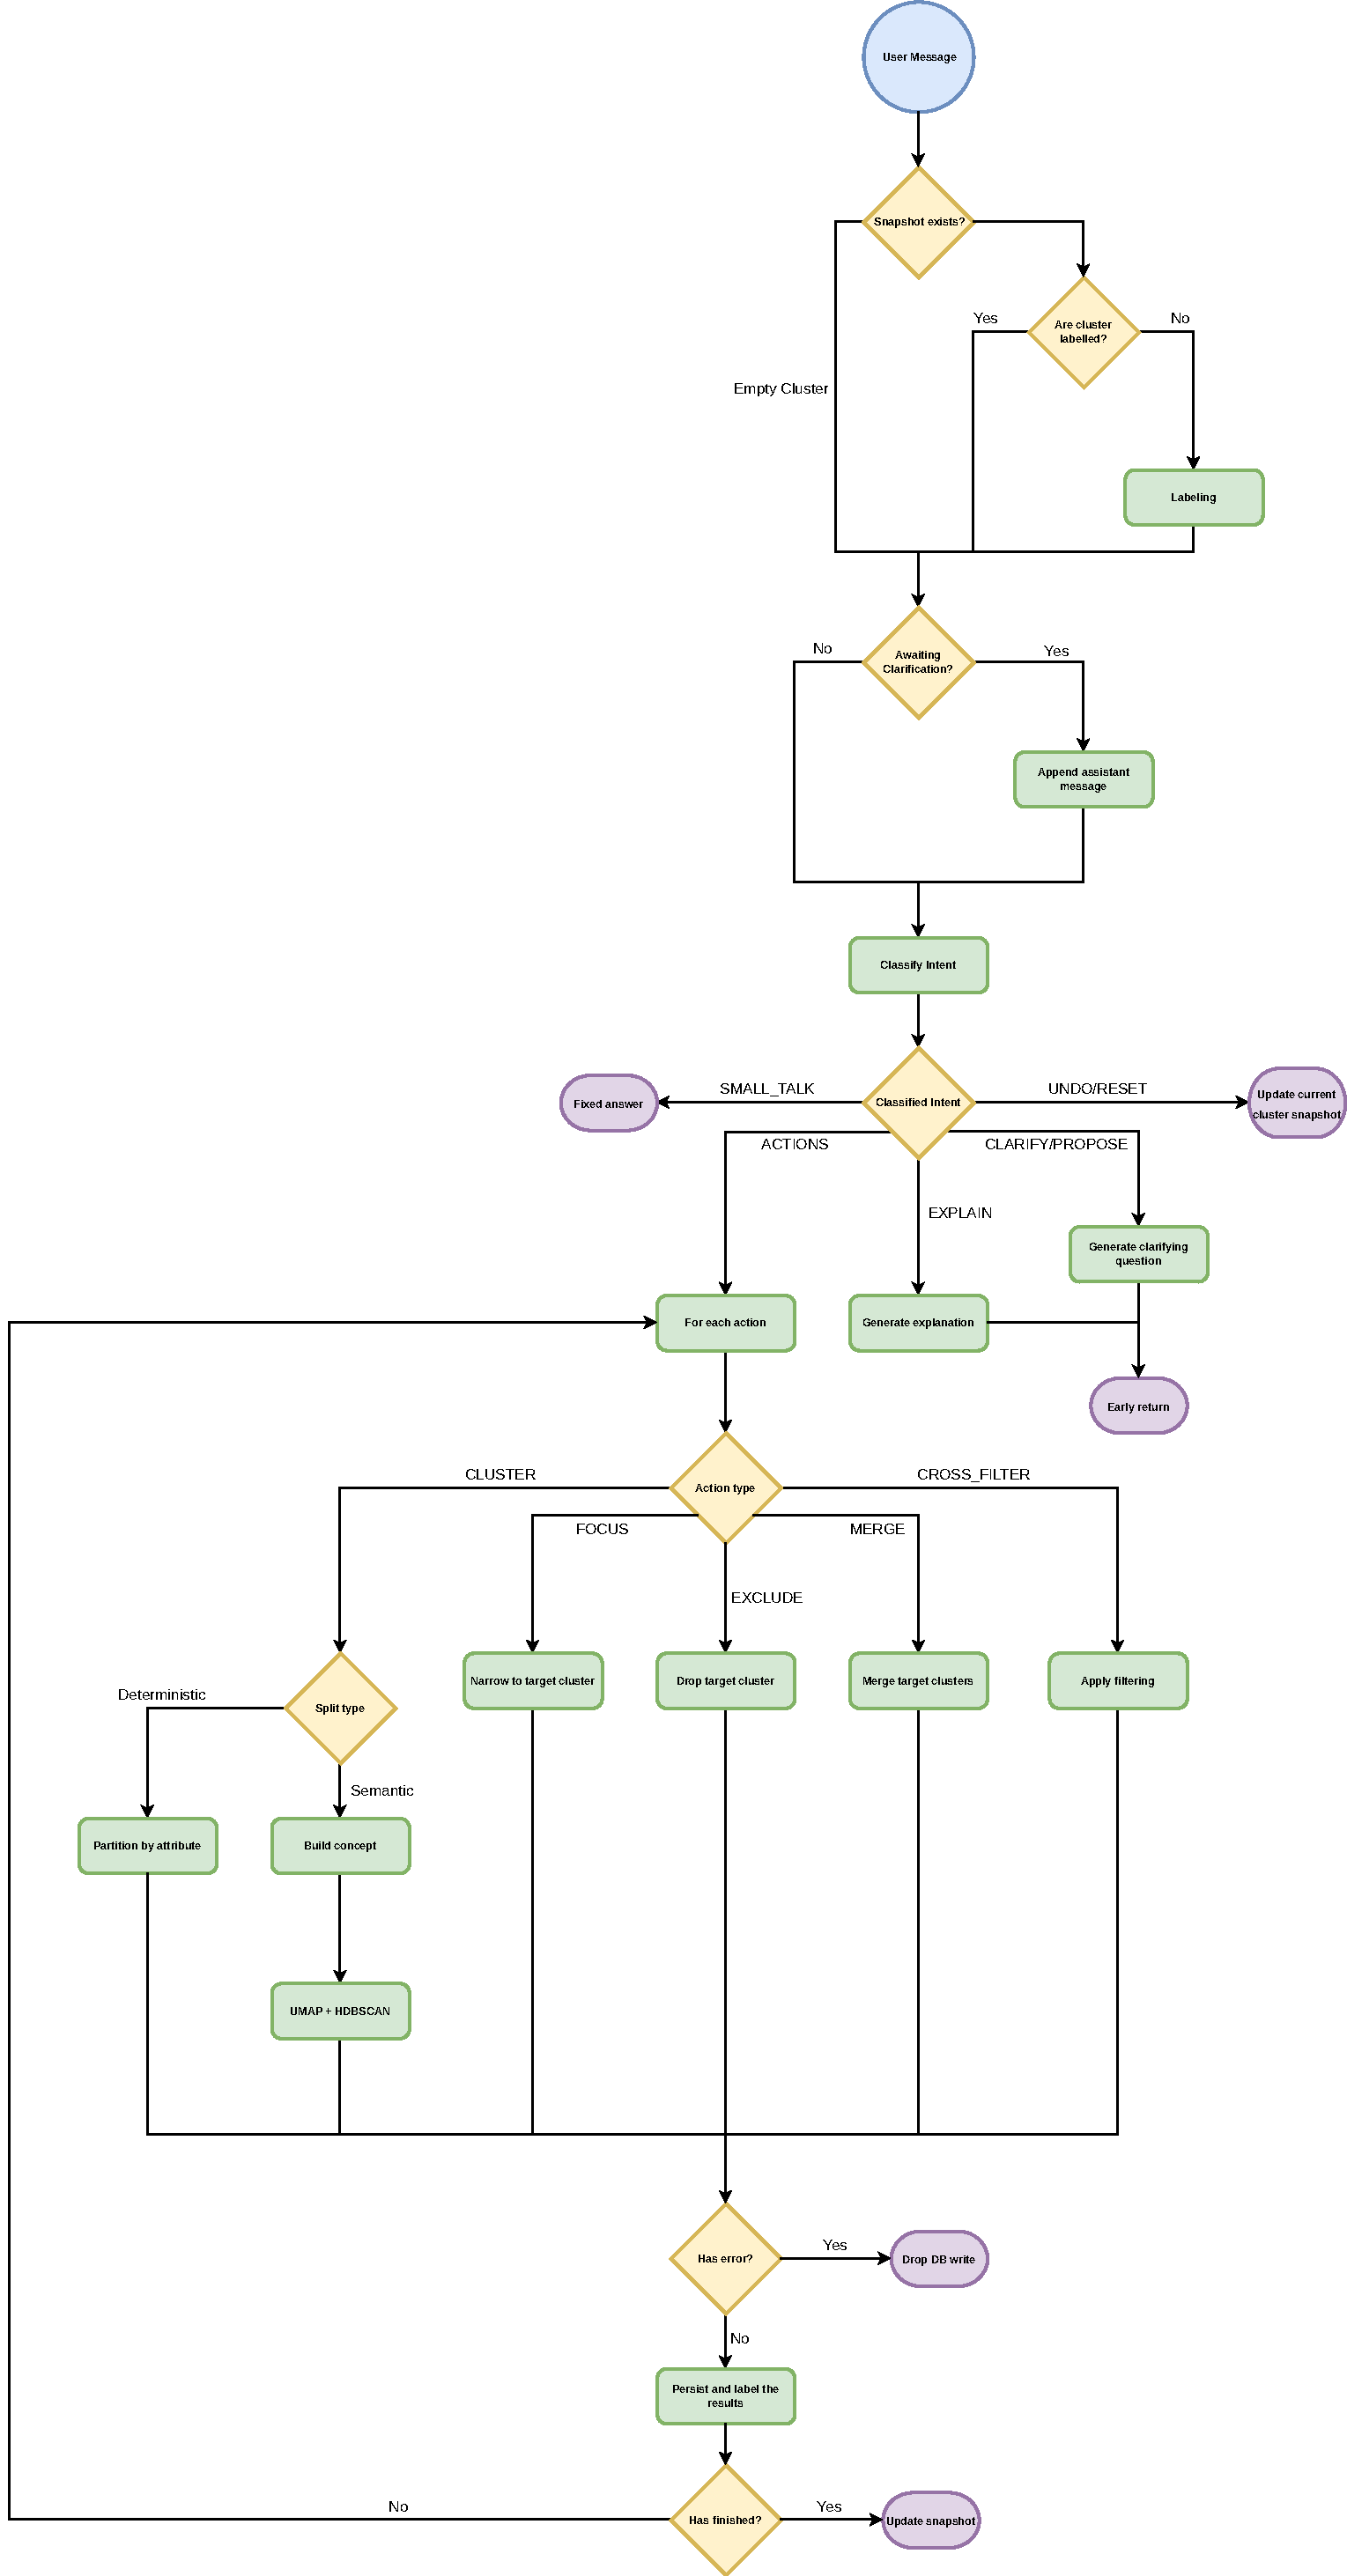
\includegraphics[height=0.92\textheight]{figures/flowchart.pdf}
  \caption{The per-turn lifecycle: load and label, resolve clarification context, classify intent,
  gate on confidence, dispatch each action to its command, and persist or drop the result.}
  \label{fig:flowchart}
\end{figure*}


\paragraph{Initialization and Intent Parsing:} The turn begins with the coordinator loading the active snapshot and labeling any remaining unlabelled clusters.
It then checks whether the previous turn ended with a clarifying question, ensuring a follow-up answer is interpreted within its proper context.
With the context established, the coordinator invokes the Intent Agent to parse the message into an ordered sequence of actions.

\paragraph{The Confidence Gate:} Before modifying any data, the system evaluates the Intent Agent's certainty.
If a state-changing action falls below the confidence threshold, the coordinator halts execution, emits a clarifying question to the oracle, and returns early without mutating state.

\paragraph{Execution and Persistence:} If the confidence gate is cleared, the coordinator dispatches the actions sequentially to their respective deterministic commands.
Each command processes the data within the state environment left by its predecessor.
The coordinator only persists the new snapshot and labels upon total success; if a command throws an error, the entire write operation is dropped. 

\paragraph{Finalization:} In the final step, the coordinator may prompt the Suggestion Agent to generate recommended next steps, aggregates the resulting response fragments, and persists the final assistant message along with its operational cost.

\paragraph{Snapshot Graph:} Rather than overwriting state data on every turn, the system records the evolution of the dialogue as a directed tree graph.
Every executed operation generates a distinct, content-addressed snapshot node containing references to its parent, the specific command executed, and its operational parameters.
Because nodes are content-addressed, arriving at an identical state via different paths automatically reuses the existing cached node.
This branching data structure natively supports advanced navigation behaviors.

\subsection{System Interfaces}

The system exposes three boundaries, all of them thin surfaces over the coordinator and the data-access layer:
\begin{itemize}[leftmargin=1.4em]
  \item \textbf{HTTP API}: carries the full session lifecycle, creating conversations, submitting messages, reading snapshots and movies, streaming per-turn progress, and serving the evaluation data, with authentication handled entirely at this layer;
  \item \textbf{Frontend}: a web application that surfaces the entire human-facing experience, from starting and replaying conversations to inspecting clusters and their member films, visualising and navigating the snapshot graph, and, for administrators, an evaluation lab that reviews run metrics, judge scores, and full transcripts;
  \item \textbf{MCP server}: re-exposes the same capabilities as a tools-only, stateless interface, so an external agent can drive CinePal exactly as a human client would.
  It deliberately stops short of the full HTTP surface, leaving out the operator and human-only concerns: authentication and per-user history, destructive hard deletes, the live progress stream, the raw UMAP projection, and the evaluation routes, none of which an autonomous client needs in order to explore the catalogue.
\end{itemize}
